% !TEX root = ../main.tex

\chapter{交流母线：10~kV 下垂调压}
\label{chap:bus}

\section{拓扑与阻抗}

实验二的对象是一台可调内部电势 $E$ 经有限阻抗向 10~kV 母线供电的三相电源，功率通路和控制结构如图~\ref{fig:droop-model} 所示。母线测点 M1 位于阻抗之后：若放在阻抗之前，控制器看到的只是自身的指令，线路压降无法被补偿，下垂调压也失去物理意义。

电网短路容量 100~MVA、$X/R=5$，由 $|Z_g|=V_b^2/S\sub{sc}=1\ \Omega$ 得
\begin{equation}
R_g=\frac{1}{\sqrt{1+5^2}}=0.196116\ \Omega,\quad
X_g=5R_g=0.980581\ \Omega,\quad
L_g=\frac{X_g}{2\pi f}=3.121285\ \mathrm{mH}.
\label{eq:zg}
\end{equation}
短路容量只用于求阻抗，控制量的标幺化以 10~MVA 为功率基准。指导书未给测试变压器参数，主验证模型补充了一台 10~MVA、Yg/Yg、10:1 的理想化变压器，漏抗、励磁和饱和均关闭，默认二次侧每相 $R_2=X_2=0.2\ \Omega$，折算到一次侧为 $20+\mathrm{j}20\ \Omega$。

\begin{figure}[htbp]
\centering
\makebox[\linewidth][c]{\begin{tikzpicture}[font=\footnotesize, >={Latex[length=1.5mm]},
  pw/.style={draw=segbus, fill=segbus!8, rounded corners=1.5pt, line width=0.6pt, align=center, minimum width=19mm, minimum height=10mm, inner sep=1pt},
  ct/.style={draw=seghb, fill=seghb!8, rounded corners=1.5pt, line width=0.6pt, align=center, minimum width=19mm, minimum height=10mm, inner sep=1pt},
  flow/.style={->, line width=0.7pt, color=black!75},
  sig/.style={->, line width=0.6pt, dashed, color=black!60}]
\node[pw] (src) at (0,0) {受控三相源\\$E\angle\delta$};
\node[pw] (zg) at (2.72,0) {电网阻抗\\$R_g,\ L_g$};
\node[pw] (m1) at (5.44,0) {测点 M1\\10~kV 母线};
\node[pw] (tr) at (8.16,0) {变压器\\10:1};
\node[pw] (m2) at (10.88,0) {测点 M2};
\node[pw] (ld) at (13.6,0) {负载\\$R_2+\mathrm{j}X_2$};
\foreach \a/\b in {src/zg, zg/m1, m1/tr, tr/m2, m2/ld}{\draw[flow] (\a)--(\b);}
\node[ct] (meas) at (5.44,-1.9) {瞬时量计算\\$v\sub{pu},\ q\sub{pu}$};
\node[ct] (filt) at (2.72,-3.5) {一阶低通\\$\tau_V,\ \tau_Q$};
\node[ct] (dr) at (5.44,-3.5) {无功下垂\\系数 0.05};
\node[ct] (pi) at (8.16,-3.5) {PI 与限幅\\$K_p,\ K_i$};
\node[ct] (ed) at (10.88,-3.5) {内电势动态\\$\tau_E$};
\node[ct] (cmd) at (13.6,-3.5) {$E\in$\\$[0.85,1.15]$~pu};
\draw[sig] (m1)--(meas);
\draw[sig] (meas.west) -| (filt.north);
\draw[sig] (filt)--(dr);
\draw[sig] (dr)--(pi);
\draw[sig] (pi)--(ed);
\draw[sig] (ed)--(cmd);
\draw[sig] (cmd.south) |- ++(-6,-0.55) -| (0,-1.3) -- (src.south);
\end{tikzpicture}}
\caption{实验二的功率通路（上）与下垂调压控制（下）：母线测点位于电网阻抗之后，控制器调节阻抗之前的内部电势}
\label{fig:droop-model}
\end{figure}

\begin{figure}[htbp]
\centering
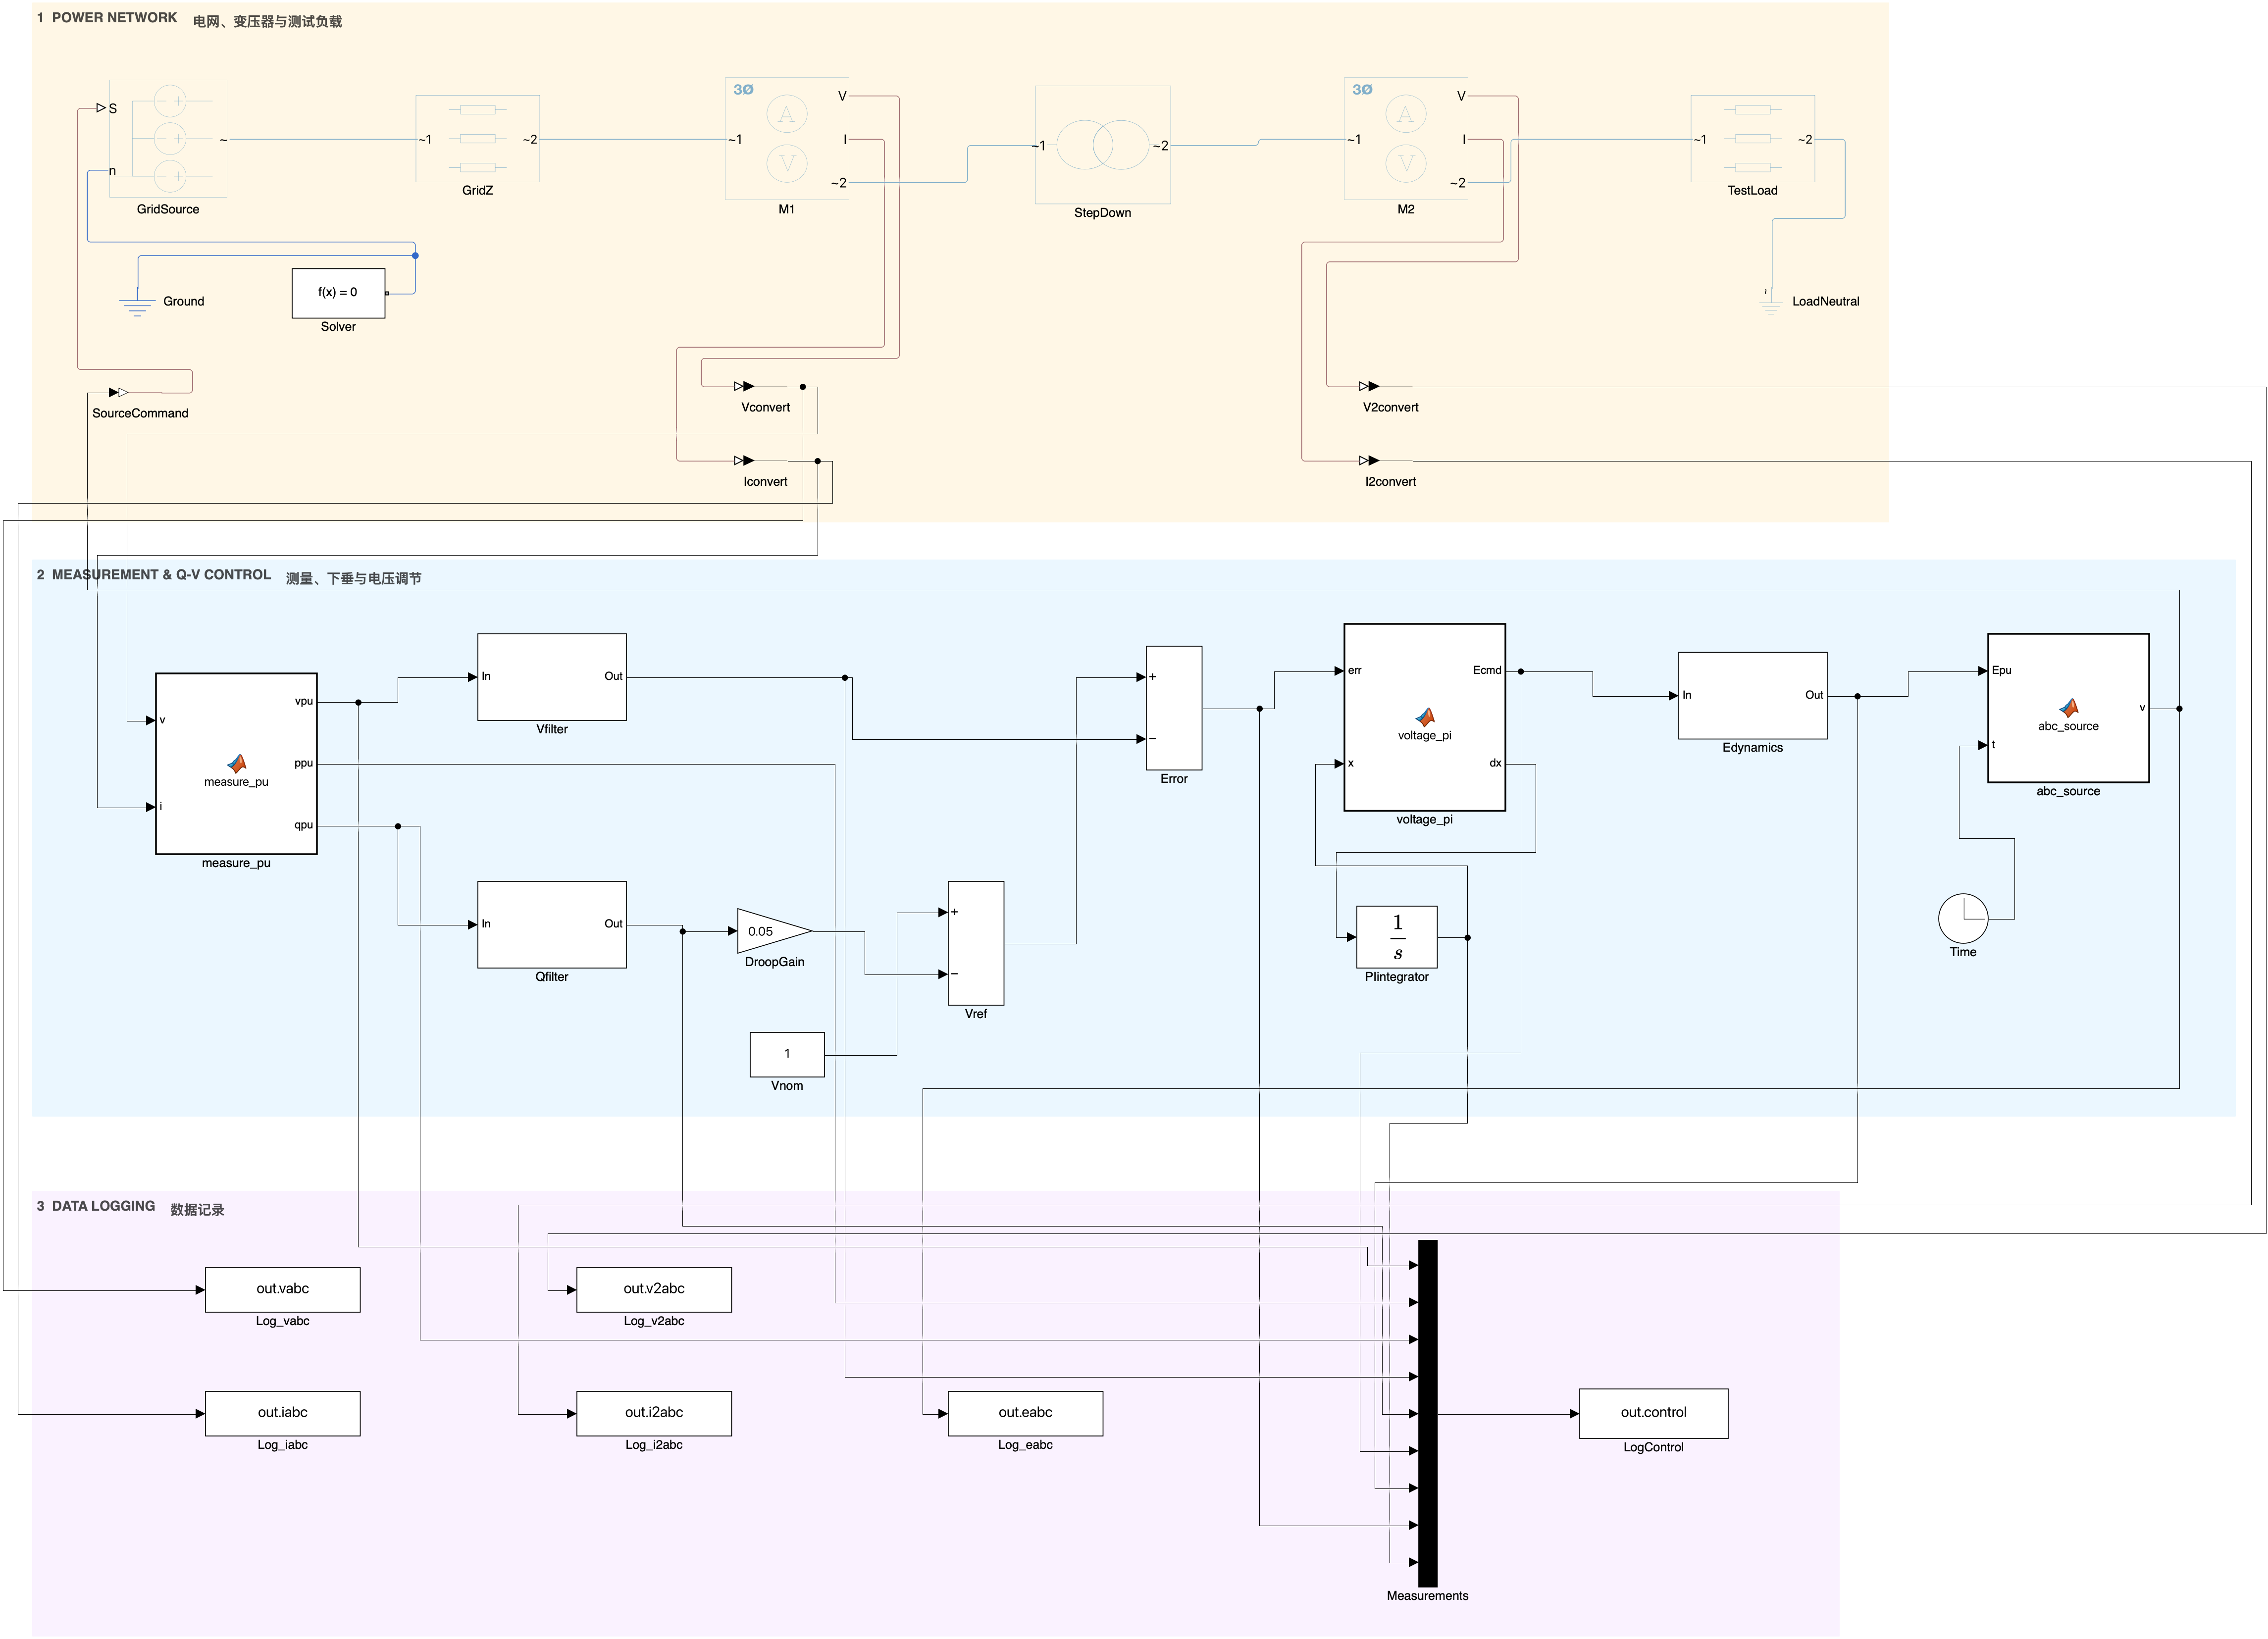
\includegraphics[width=0.62\linewidth]{native/model_droop.png}
\caption{实验二模型顶层（Simulink 原生视图）：电气网络、测量与下垂调压、数据记录三个分区}
\label{fig:droop-native}
\end{figure}

\section{测量与控制}

M1 输出三相瞬时电压和电流。取等幅值 Clarke 变换
\begin{equation}
v_\alpha=\frac{2}{3}\Bigl(v_a-\frac{v_b}{2}-\frac{v_c}{2}\Bigr),\qquad
v_\beta=\frac{\sqrt3}{3}(v_b-v_c),
\end{equation}
电流同理，并按瞬时功率理论\cite{akagi2007}计算标幺量：
\begin{equation}
v\sub{pu}=\frac{\sqrt{1.5(v_\alpha^2+v_\beta^2)}}{10^4},\quad
p\sub{pu}=\frac{v_ai_a+v_bi_b+v_ci_c}{10^7},\quad
q\sub{pu}=\frac{1.5(v_\beta i_\alpha-v_\alpha i_\beta)}{10^7}.
\label{eq:pq}
\end{equation}
平衡正弦条件下 $v\sub{pu}$ 即线电压有效值相对 10~kV 的标幺值，感性负载给出正无功。

电压、无功和内部电势各经一阶环节，时间常数为 $\tau_V=0.01$~s、$\tau_Q=0.02$~s、$\tau_E=0.05$~s。无功下垂给出电压目标\cite{kundur1994}
\begin{equation}
v\sub{ref}=1-0.05\,q\sub{f}.
\label{eq:droop}
\end{equation}
电压误差 $e=v\sub{ref}-v\sub{f}$ 送入 PI 控制器（$K_p=0.5$，$K_i=10\ \mathrm{s^{-1}}$），输出限幅后加在 1 上得到内部电势指令 $E\sub{cmd}\in[0.85,1.15]$~pu。抗饱和采用条件积分：控制器处于限幅且误差继续朝饱和方向时积分增量置零，误差反向后积分立即恢复。

限幅对象是阻抗之前的内部电势。轻中载时控制器可以抬高 $E$ 补偿 $Z_g$ 上的压降，$E$ 触及 1.15~pu 后母线电压就无法继续抬升。这一点是第 \ref{chap:analysis} 章接口核算的关键。

\section{独立相量解}

为避免仿真自证，另外写出不经过 Simulink 积分器的稳态相量解。令 $Z_t=Z_L+100(Z_2+r_w)$（$r_w$ 为微小绕组电阻），负载无功写成 $q\sub{pu}=cV\sub{pu}^2$，其中 $c=10\,\mathrm{Im}(Z_L)/|Z_t|^2$。未限幅时稳态同时满足式~\eqref{eq:droop}，解得
\begin{equation}
V\sub{pu}=\frac{2}{1+\sqrt{1+0.2c}},\qquad
E\sub{req}=V\sub{pu}\frac{|Z_g+Z_t|}{|Z_t|}.
\label{eq:phasor}
\end{equation}
若 $E\sub{req}>1.15$~pu，则把源电势固定在上限，再按电压分配重算母线电压。

\section{六个工况的结果}

图~\ref{fig:bus-response} 给出默认工况的启动过程和稳态三相波形。默认工况下母线先因 $Z_g$ 压降下降，无功经低通后逐渐建立，$v\sub{ref}$ 降到约 0.9878~pu，PI 同时把 $E$ 抬到 1.0170~pu，$v\sub{f}$ 与 $v\sub{ref}$ 重合，说明未限幅时闭环无差。末段 $V\sub{bus}=0.987803$~pu，而由 $Q/S_b=0.243938$ 计算的下垂目标为 0.9878031~pu，两者相差 $3.9\times10^{-12}$~pu。

三相波形在 1.94--2.00~s 内平衡、周期 20~ms。一次线电压有效值 9877.83~V，二次侧 987.783~V，比值 10.000；相邻相相位差为 $-120.00002^\circ$ 和 $-119.99998^\circ$，三相电压和的峰值为 $8.5\times10^{-8}$~V，没有共模偏置。

\twofig{native/bus_voltage_power.pdf}{native/bus_three_phase.pdf}{默认 RL 工况的 MATLAB 原生波形：(a) 启动段电压与功率，(b) 稳态三相相电压}{fig:bus-response}

\begin{figure}[htbp]
\centering
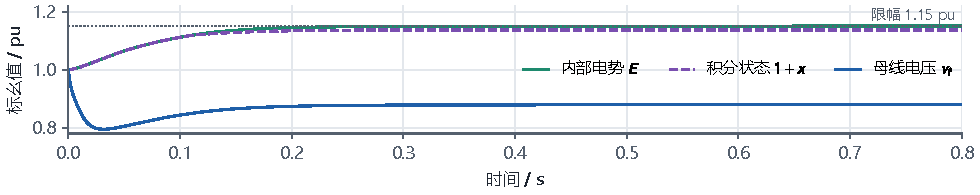
\includegraphics[width=\linewidth]{bus_saturation}
\caption{零积分初值重载工况：内部电势触及限幅后积分状态冻结，母线停在 0.8786~pu}
\label{fig:bus-sat}
\end{figure}

表~\ref{tab:bus-cases} 是六个工况的末段时间平均值。近空载和纯电阻工况 $Q\approx0$，目标为 1~pu，纯电阻工况为克服有功电流的线路压降把 $E$ 升到 1.011~pu。从默认 RL 到较强感性，$Q$ 由 2.44~Mvar 升到 3.85~Mvar，母线按下垂规律由 0.9878~pu 降到 0.9808~pu。

\begin{dtable}{htbp}{六个工况的稳态结果与独立相量解偏差}
\label{tab:bus-cases}
\begin{tabularx}{\linewidth}{LRRRRR}
\toprule
\headrow 工况 & $V\sub{bus}$ / pu & $P$ / MW & $Q$ / Mvar & $E$ / pu & $|\Delta V|$ / pu \\
\midrule
近空载 & 1.000000 & 0.00100 & 0.00000 & 1.000002 & $6.4\times10^{-8}$ \\
纯电阻 & 1.000000 & 4.99999 & 0.00000 & 1.010995 & $9.1\times10^{-8}$ \\
默认 RL & 0.987803 & 2.43934 & 2.43938 & 1.017047 & $2.8\times10^{-8}$ \\
较强感性 & 0.980762 & 1.92375 & 3.84754 & 1.023143 & $1.6\times10^{-7}$ \\
零初值重载 & 0.878646 & 19.30053 & 19.22465 & 1.150000 & $7.8\times10^{-5}$ \\
默认 RL 半步长 & 0.987803 & 2.43938 & 2.43938 & 1.017046 & $2.5\times10^{-9}$ \\
\bottomrule
\end{tabularx}
\end{dtable}

零初值重载是唯一撞限幅的工况（图~\ref{fig:bus-sat}）。负载折算到一次侧只有 $2+\mathrm{j}2\ \Omega$，稳态所需内部电势超过 1.15~pu。$E\sub{cmd}$ 在 0.110525~s 首次触及上限，此后 $E$ 按 $\tau_E$ 平滑跟随；积分状态涨到 0.137388~pu 后冻结。母线最终落在 0.878646~pu，比下垂目标 0.903877~pu 低 0.025230~pu，这一残余误差反映电源能力不足，与 PI 参数无关。

默认工况把最大步长由 $5\times10^{-5}$~s 减半后，母线末段均值只变化 $2.53\times10^{-8}$~pu，相量偏差由 $2.8\times10^{-8}$~pu 降到 $2.5\times10^{-9}$~pu，结果与步长无关。

100~MVA 短路容量与 2.44~MW 负载之比为 41，属于很强的母线，所以默认工况电压只下降 1.2\%。这一判断只对该负载成立，第 \ref{chap:analysis} 章将说明它不能外推到实验一的 59.6~MW。
